% Please do not change the document class
\documentclass{scrartcl}

% Please do not change these packages
\usepackage[hidelinks]{hyperref}
\usepackage[none]{hyphenat}
\usepackage{setspace}
\doublespace

% You may add additional packages here
\usepackage{amsmath}
\usepackage{float}
\usepackage{graphicx} 
\graphicspath{ {Diagrams/} }

% Please include a clear, concise, and descriptive title
\title{COMP310 Proposal}

% Please do not change the subtitle
\subtitle{COMP310}

% Please put your student number in the author field
\author{1507866}

\begin{document}
	
\maketitle
\section{What is the title of the game?}
?????
\section{On what well-known game is it based?}
My de-make will be based off of Mirror's Edge. 

\section{What is the core mechanic that your game will implement?}
The core mechanic of Mirror's Edge is parkour. For this de-make I'll simplify this to moving left and right, jumping and crouching. The player will be able to move through the cityscape and jump on buildings. 
A stretch goal is to add enemies, these enemies will probably not move and the player will be able to jump over them or on them to defeat them. 

\section{Is the game technically feasible, given the limitations of the target platform?} \textit{Make reference to existing NES games and to technical documentation.}

Looking at existing NES games it seems technically feasible. Super Mario Bros and Kirby's Adventure both have scrolling backgrounds but to avoid graphical glitches I'll only let the background scroll in one direction.
Mirror's Edge also has a limited colour pallete, most environments are focused on a single colour which should fit well with the limited colour pallete.

\begin{figure}[H]
	\centering
	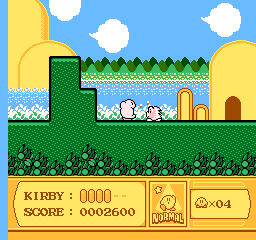
\includegraphics[width=0.5\linewidth]{Kirby.PNG}
	\caption{Kirby's Adventure for NES }
\end{figure}
	
\begin{figure}[H]
	\centering
	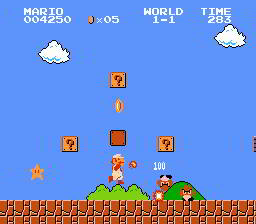
\includegraphics[width=0.48\textwidth]{mario.JPG}
	\caption{Super Mario Bros for NES }
\end{figure}


\section{What is the intended aesthetic?}
Sidescrolling platform game.


\begin{figure}[H]
	\centering
	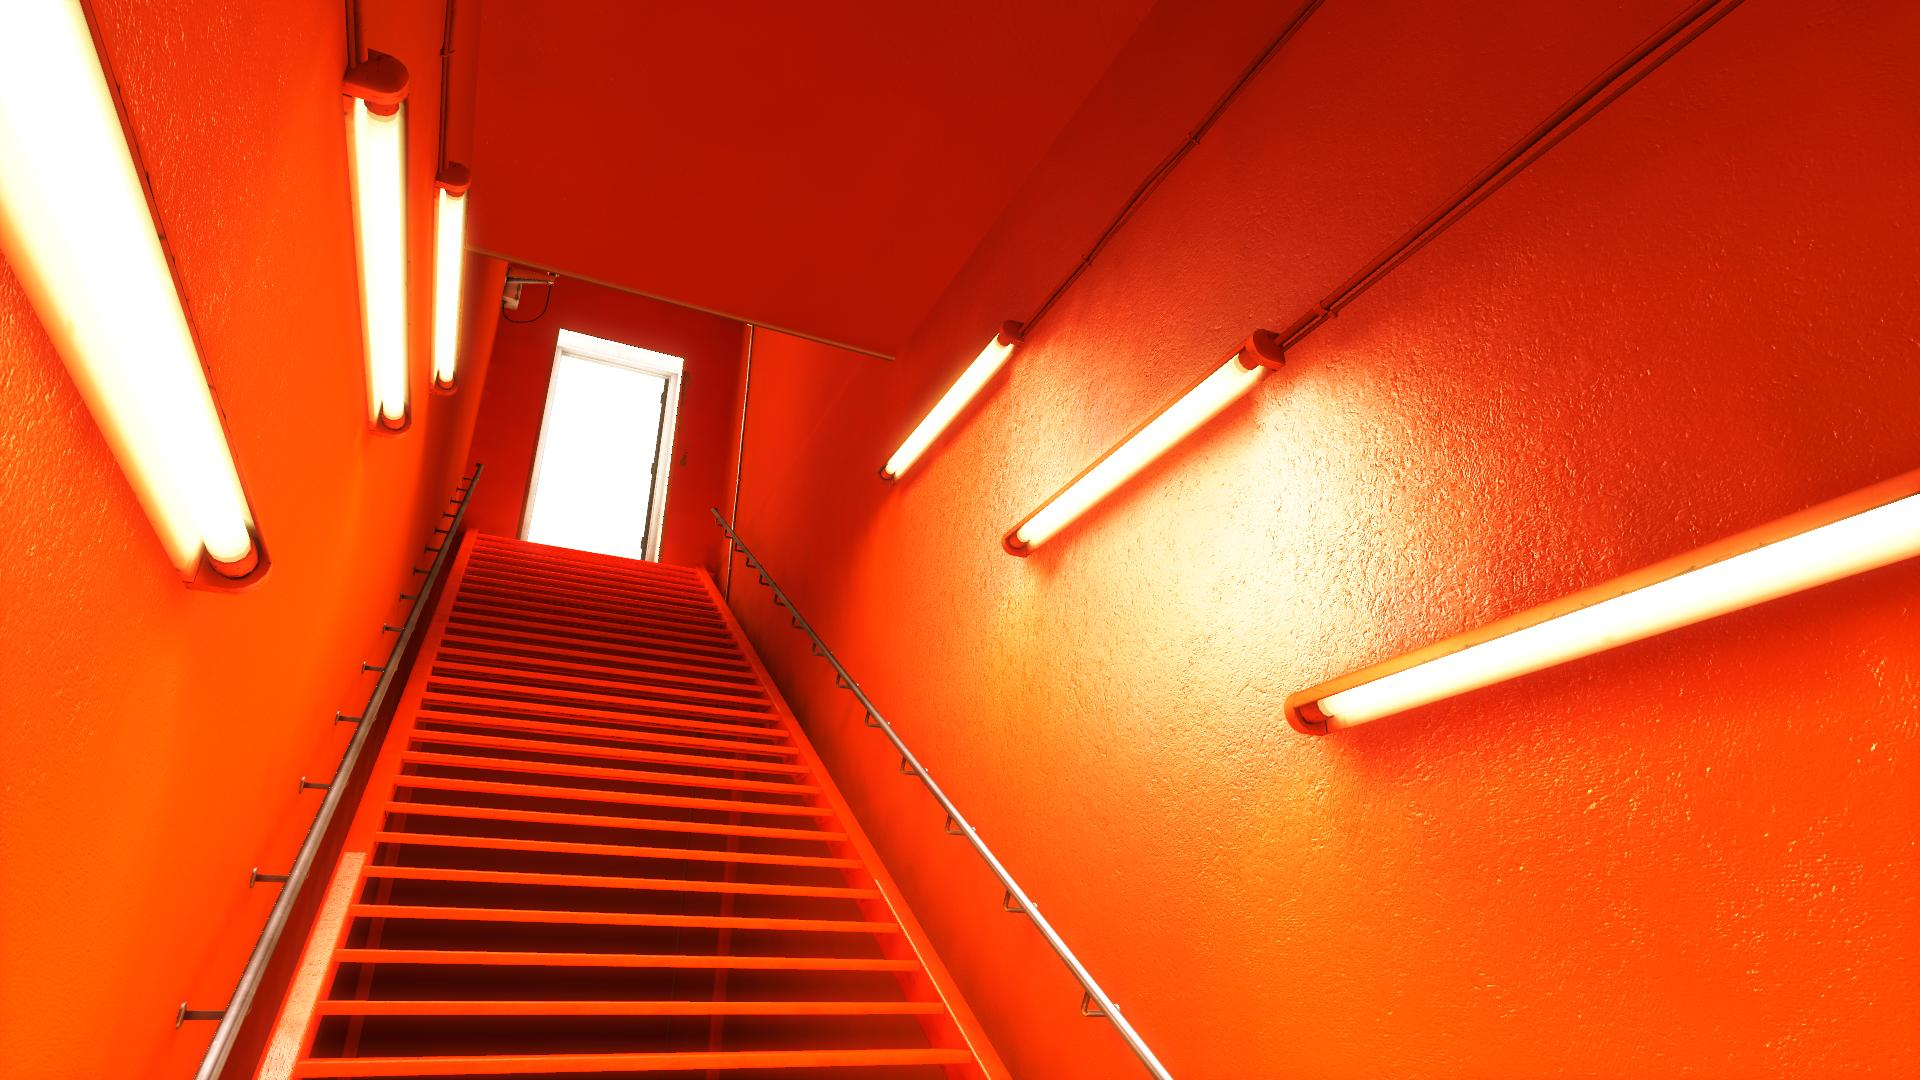
\includegraphics[scale=0.15]{MEO.jpg}
	\caption{Mirror's Edge - Orange Area}
	
\end{figure}

\begin{figure}[H]
	\centering
	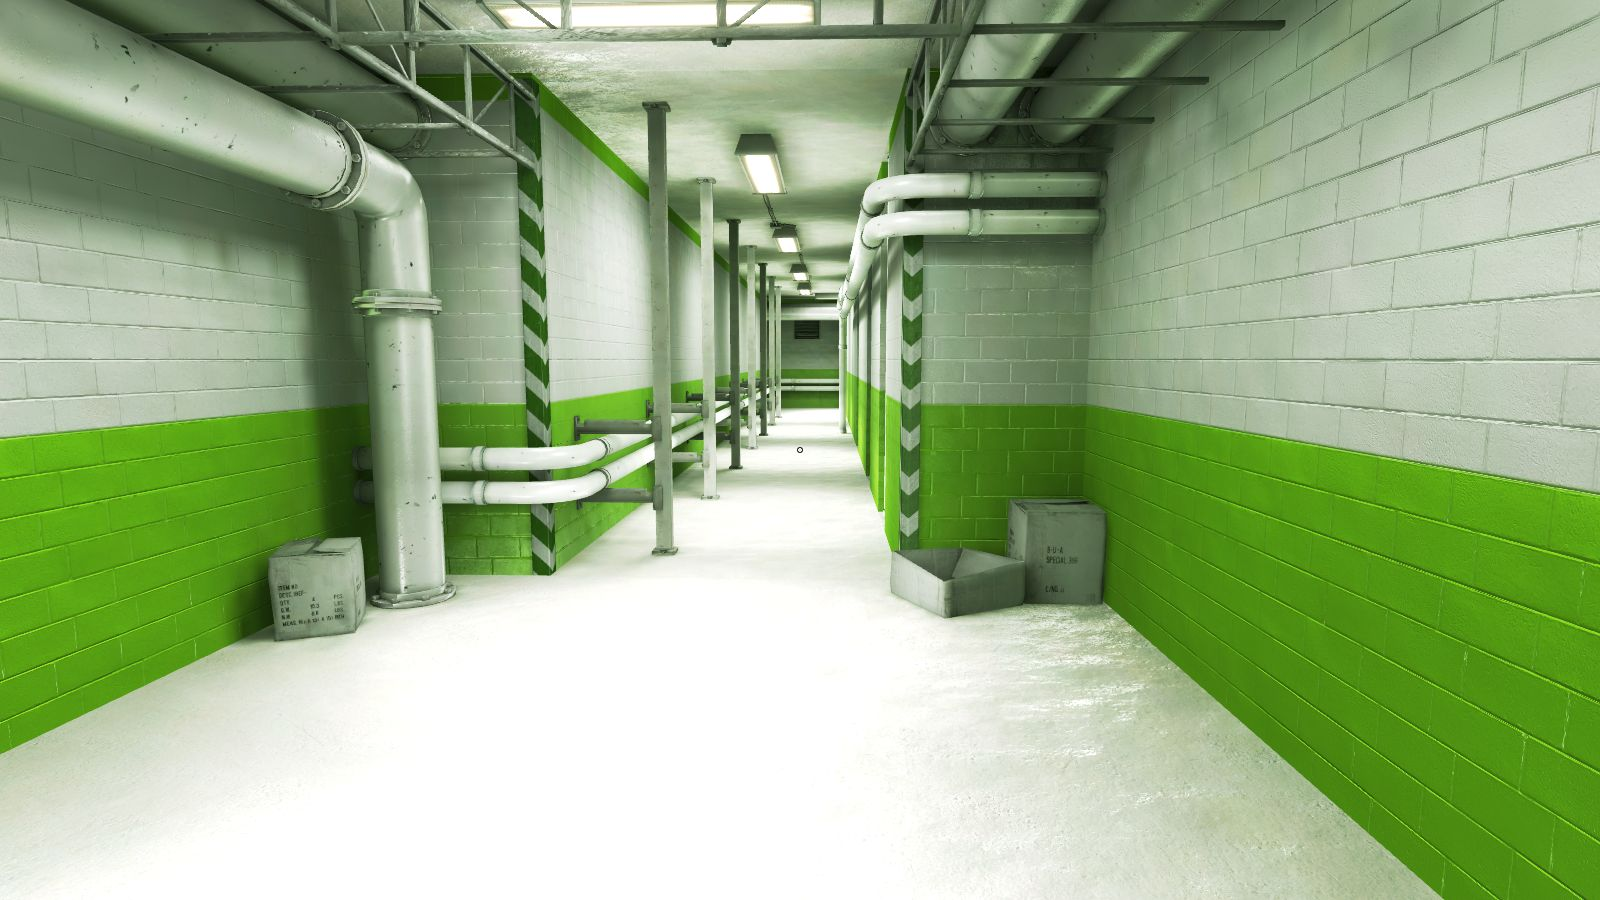
\includegraphics[scale=0.2]{MEG.jpg}
	\caption{Mirror's Edge - Green Area}
\end{figure}

\section{Is the scope appropriate for the product development time-frame?}
I think the game is fairly easy to scope up or down depending on how difficult I find it. 
	
\end{document}